Com base nos problemas identificados no processo do MOA, foi construído um Diagrama de \emph{Fishbone}, conforme descrito na Figura \ref{fig:fishbone}, de maneira a possibilitar uma boa percepção do problema principal e das causas raízes.
\begin{landscape}
	\vspace*{\fill}
	\begin{figure}[H]
		\centering
		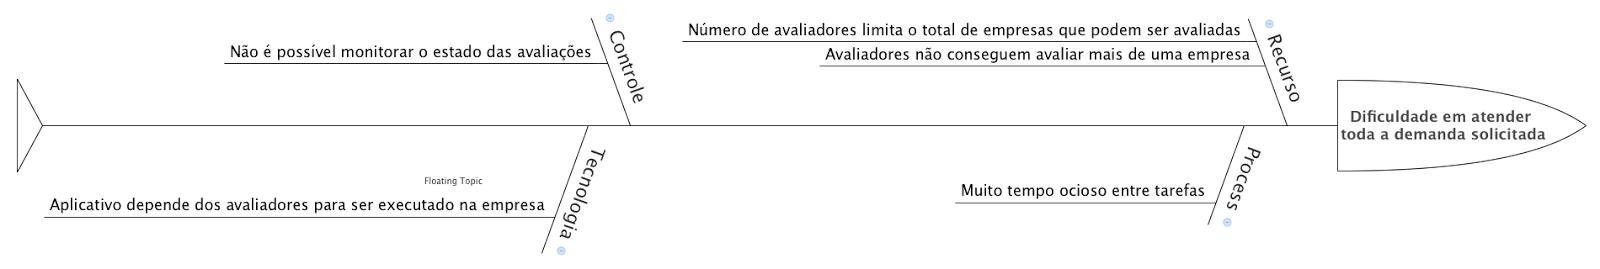
\includegraphics[scale=0.55]{fishbone}
		\caption[Diagrama de Fishbone]{Diagrama de Fishbone.}
		\label{fig:fishbone}
	\end{figure}
	\vspace*{\fill}
\end{landscape}